\documentclass{beamer}

\usepackage[T1]{fontenc}
\usepackage[utf8]{inputenc}
\usepackage[french]{babel}
%\usepackage{pslatex}
%\usepackage{colortbl}
%\usepackage{calc}
\usepackage{graphicx}
\usepackage{hyperref}
\usepackage{listings}

\lstset{language=bash,basicstyle=\ttfamily}

\usetheme{Warsaw}

\newcommand{\git}{\texttt{git}}

\definecolor{fondtitre}{rgb}{0.20,0.43,0.09}  % vert fonce
\definecolor{coultitre}{rgb}{0.41,0.05,0.05}  % marron
\definecolor{fondtexte}{rgb}{1,1,1}           % fond blanc
\definecolor{autre1}{RGB}{250,150,5}          %vieux mauve
\definecolor{autre2}{RGB}{235,175,235}        %horrible r
\colorlet{coultexte}{black}

\setbeamercolor{structure}{fg=coultitre, bg=fondtitre!40}
\setbeamercolor{block body}{bg=fondtexte}
\setbeamercolor{normal text}{fg=coultexte,bg=fondtexte}

\setbeamertemplate{navigation symbols}{} 

\setbeamertemplate{footline}{
  \hbox{
    \hspace*{-0.06cm}

    \begin{beamercolorbox}[wd=.3\paperwidth,ht=2.25ex,dp=1ex,center]{title in head/foot}
      \usebeamerfont{author in head/foot}\insertshortauthor
      \end{beamercolorbox}

      \begin{beamercolorbox}[wd=.4\paperwidth,ht=2.25ex,dp=1ex,center]{title in head/foot}
      \usebeamerfont{title in head/foot}\insertshorttitle
      \end{beamercolorbox}

      \begin{beamercolorbox}[wd=.1\paperwidth,ht=2.25ex,dp=1ex,center]{date in head/foot}
      \usebeamerfont{date in head/foot}
    \insertframenumber{} / \inserttotalframenumber\hspace*{2ex}
    \end{beamercolorbox}

      \begin{beamercolorbox}[wd=.2\paperwidth,ht=2.25ex,dp=1ex,center]{date in head/foot}
      \usebeamerfont{date in head/foot}\insertdate
      \end{beamercolorbox}}

      \vskip0pt
}

\title[ROSE]{Gestion de versions : \git}
\author{Bertrand, Clément, Laurent, Vaibhav.}
\institute{Télécom ParisTech}
\date{4 mars 2011}

%---------------------------------------

\begin{document}

\begin{frame}
  \titlepage
\end{frame}

%------------------ Plan ---------------
\section*{Plan}
\frame{\frametitle{Plan} \small \tableofcontents}

%------------------ Slides ------------
\section{Introduction}
\subsection*{Présentation des objectifs}
\begin{frame}{Présentation des objectifs}
  \begin{itemize}
  \item Comprendre ce qu'est un gestionnaire de version et son utilité
  \item Connaître les commandes de bases pour se débrouiller
  \item Avoir des éléments de compréhension sur le fonctionnement de \git
  \item Savoir où chercher en cas de problèmes
  \end{itemize}
\end{frame}

\subsection*{Logiciels de gestion de versions}
\begin{frame}{Logiciels de gestion de versions}
  \begin{itemize}
  \item Garde une trace des différentes versions d'un projet
  \item Facilite le travail en équipe grace aux branches
  \item Se couple avec des logiciels qui permettent de comparer les différences entre fichiers
  \item Permet la résilience aux pannes suivant que le système est distribué ou non
  \item Peut être distribué ou non : \git est distribué
  \end{itemize}
\end{frame}

\section{Installer et configurer \git}

\subsection*{Installation}
\begin{frame}{Installation}
  \begin{itemize}
  \item paquets à installer (debian/ubuntu) :
  \item windows :
  \item mac :
  \end{itemize}
\end{frame}

\subsection*{Configuration}
\begin{frame}[containsverbatim]{Configuration}
  \begin{itemize}
  \item fichier de configuration \lstinline|~/.gitconfig| ou en ligne de commande \lstinline|git config|
  \item
  \end{itemize}
\end{frame}

\section{Les bases de \git}
\subsection*{Statut de fichiers}
\begin{frame}{Statut de fichiers}
  \begin{figure}
    \begin{center}
      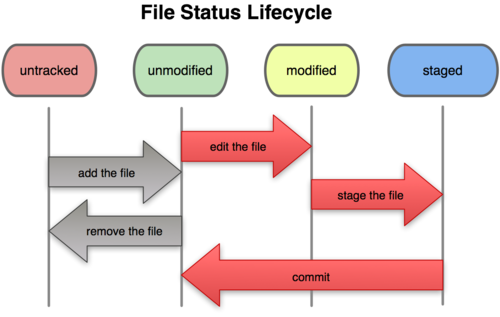
\includegraphics[scale=0.7]{img/Status_lifecycle.png}
    \end{center}
    \caption{progit.org}
  \end{figure}
\end{frame}

%------------------------------------------------------------
% Clément & Bertrand


\section{Le Branching}
\subsection*{Gestion Locale}
\begin{frame}{Gestion Locale 1/2}
  \begin{figure}
    \begin{center}
      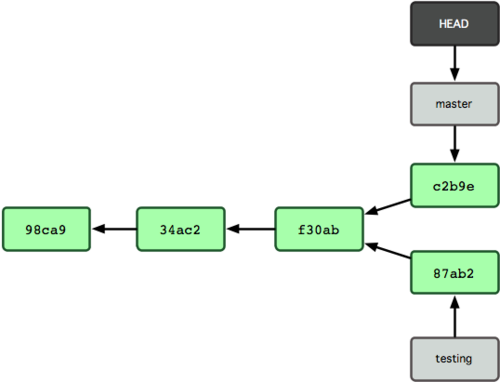
\includegraphics[scale=0.7]{Branch1.png}
    \end{center}
    \caption{progit.org}
  \end{figure}
\end{frame}

\begin{frame}{Gestion Locale 1/2}
  \begin{itemize}
  \item Lister les branches : \emph{git branch}  
  \item Lister les branches mergées avec la branche courante : \emph{git branch}
  \item Lister les branches non mergées avec la branche courante : \emph{git branch}  
  \item Lister les branches : \emph{git branch}  
  \item Créer une branche : \emph{git branch <name>}
  \item Supprimer une branche : \emph{git branch -d <name>}
  \item Déplacer HEAD vers branch : \emph{git checkout <branch>}
  \item Création et déplacer HEAD : \emph{git checkout -b <branch>}
  \item Log, dernier commit de chaque branche : \emph{git branch -v}
  \end{itemize}
\end{frame}

\subsection*{Communication avec le serveur}
\begin{frame}{Communication avec le serveur 1/2}
  \begin{itemize}
  \item Fetch
  \item Push
  \item Pull
  \item Tracking : push -u / checkout --track / git checkout -b
  \end{itemize}
\end{frame}

\begin{frame}{Communication avec le serveur 2/2}
  \begin{figure}
    \begin{center}
      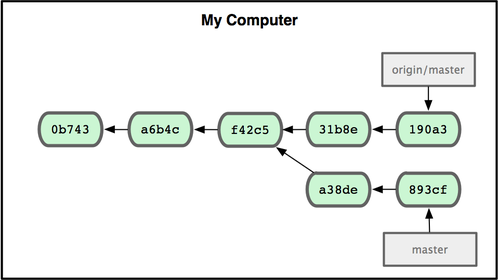
\includegraphics[scale=0.7]{RemoteBranch.png}
    \end{center}
    \caption{progit.org}
  \end{figure}
\end{frame}

\subsection*{Merger}
\begin{frame}{Merger 1/2}
  \begin{itemize}
  \item Merge
  \end{itemize}
\end{frame}

\begin{frame}{Merger 2/2}
  \begin{figure}
    \begin{center}
      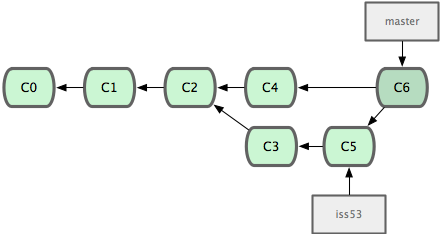
\includegraphics[scale=0.7]{Merge.png}
    \end{center}
    \caption{progit.org}
  \end{figure}
\end{frame}

\subsection*{Rebase}
\begin{frame}{Rebase 1/2}
  \begin{itemize}
  \item
  \end{itemize}
\end{frame}

\begin{frame}{Rebase 2/2}
  \begin{figure}
    \begin{center}
      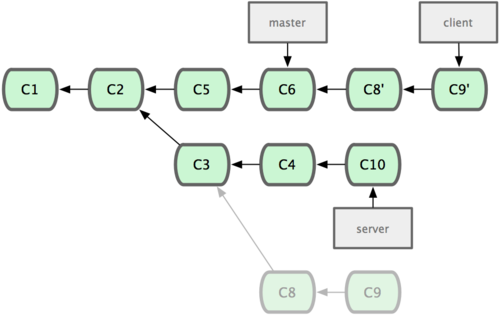
\includegraphics[scale=0.7]{Rebase.png}
    \end{center}
     \caption{progit.org}
  \end{figure}
\end{frame}
%------------------------------------------------------------

\section{Ressources}
\begin{frame}{Ressources}
  \begin{itemize}
  \item \href{http://progit.org/about.html}{Progit}
  \item \href{http://git.or.cz/gitwiki/GitHosting}{Liste de serveurs \git}
  \end{itemize}
\end{frame}

\end{document}
